\section{User Manual}\label{app:UserManual}
\newcommand{\guide}[3][\linewidth]{
\begin{figure}[H]
    \centering
    \includegraphics[page=#2, width = #1]{.Figures/Guide.pdf}
    \caption{#3}
\end{figure}
}

\newcommand{\note}[1]{
\begin{figure}[H]
\noindent\hrulefill 

\textit{Note: #1}\vspace{-1mm}

\noindent\hrulefill
\end{figure}
}

This guide explains how a user can interact and use the program, to perform an LCA analysis on a system. This program assumes that the unit processes in the system are expressed in terms of their impact categories, defined by an LCIA model. It does not take elementary flows as input directly. Existing tools are capable of performing this characterisation for us.

When the program is started, the first window encountered is the home window. 
\guide[0.95\linewidth]
{1}{Home Window.}

\note{We will reference the different branches (defined in the design section) as windows, as this is common when explaining the layout of a program, although they are in fact implemented as \texttt{Frames} embedded in a single window.}

In the home window, the main logo for the program is shown. At the top, there is a ribbon containing buttons for navigating the different windows in the program. At the bottom it is possible to load and save the created LCI model. 

Loading and saving a model is done using a file-chooser dialog. Here the user chooses the desired files for the action. The file-chooser dialog is seen here, while attempting to load a model with the \texttt{ReCiPe} method defined.

\guide[0.8\linewidth]
{2}{File-chooser-dialog for loading and saving.}

When loading a model, the current model of the program is substituted with the loaded model. This is to keep components separated, which do not belong together.

From the home window, the natural next step is to navigate to the impact categories window. In this window the user can specify which impact categories the system will be expressed in, and save them as an LCIA method.

\guide
{3}{LCIA Method Window.}

The loaded LCIA method is seen here, with the method name and the categories defined. For each category we have the name and unit specified. 

This method is saved, and therefore cannot be changed. This ensures that a method is not altered, after components are created based on it.

It is possible to create a new LCIA method once a name is entered in the top entry. Once a new method is created, the remaining buttons will be enabled and the 'Select Method' button will be disabled. Methods are not stored in the model before they are explicitly saved. All categories in the LCIA method are required to have unique names, and thus the method cannot be saved until this requirement is satisfied.

Adding impact categories to a method can either be done using the 'Add Category' button, which adds a single category with the default name 'Name' and unit 'Unit', which can be changed as desired as long as the method is not saved. Alternatively impact categories can be defined in bulk by the 'Add Multiple Categories'. Here a data prompt window will open up, where the category names and units can be entered.

\guide[0.5\linewidth]
{4}{Data Prompt Window, for entry of multiple data values.}

The information entered in the data prompt window is parsed as tab-separated columns.\footnote{Empty columns are ignored} If two columns of are entered, the values will be inserted as categories with names and units respectively. If a single column is entered, the values will be inserted as categories with the specified values as names, but with a default unit of 'Unit'. If no data is entered it is equivalent to pressing the 'Add Category' button. Categories can be removed by the 'Remove Category' button. After creating and selecting an LCIA method, we can begin defining our systems.

\guide
{5}{Background Systems Window.}
Firstly we will look at the background systems. Similar to when we created the LCIA method, we create the background system by typing the name in the top entry and pressing the 'New Background System' button.

Once created, it is possible to define unit processes for the background system in a similar fashion. Creating a unit process adds a process to the background system with the default usage of '1'. The unit process can be seen in the view below the 'New Unit Process' button, and when pressed, the defining impact quantities are seen in the center/main view. Note that impact quantities for each of the impact categories in the LCIA method is created automatically.

The usage of the unit process and the impact quantities for its categories can be changed directly in the view, but only for the base time step (being the first defined time step with default value '0'). 

\note{Time steps for the different components are defined by decimal values, and are all defined by the same unit. This way there are no assumptions regarding leap-year, month length, 12h/24h etc.}

To define the dynamic properties of the components, the three data buttons are used; 'Add Background System Data', 'Add Unit Process Data' and 'Add Impact Data'. These buttons open windows for each of the respective components and their properties.

\guide[0.8\linewidth]
{6}{Dynamic Background System Data Window.}
In the 'Background System Dynamic Data Window' it is possible to define the usage of each internal unit process and the general dynamic property for the background system. 

To enter a usage for a unit process, the desired unit process is chosen in the combobox in the top middle, where the default usage of 'Timestamp: 0, Usage: 1' is seen. These values can be changed directly in the view. Adding usages can be done either individually or in multiple at the time (similar to previously). Adding individual usages creates entries with default values. Adding multiple usages happens using the same data prompt, where a single column of data is added as usages with the values as their time stamps but with default usage of '1', and two columns are added as usages with time stamps and usages as the respective values. Again if no data is entered, it results in the insertion of a single default usage. Usages can be removed from the unit processes by the 'Remove Usage' button.

Using the 'Interpolate between usages' checkbox it is possible to define if the intermediate usages should be interpolated, or based on last known usage when requesting such time steps during calculations.

\note{
Usages with the same time stamps are overwritten when applied, as time stamps are kept unique. Only the last defined usage in that time stamp is stored.}

The general dynamic property for the background system is added with the default values of 'start:0, f(t,q): "", end: 0'. This function is equivalent to the identity function. The values can be changed in the view. The dynamic property will be active in the specified interval, and is defined as a piece-wise function. For continuation, the piece-wise function is implemented by applying the next function piece from where the previous ended. This makes it easier to model continuously changing systems.

An example of a function piece is 'start: 0, f(t,q): "q*0.95{\textasciicircum}t", end: 100', which express a 5\% decrease from time step 0 to 100. Function pieces can be removed by the respective button.

\note{
When entering values in views, the data is saved when the cell is no longer edited (i.e. is exited). For data windows it is therefore important that cells are finished before applying the changes.}

\guide[0.7\linewidth]
{7}{Dynamic Unit Process Data Window.}
Similar to general dynamic properties for the background system, it is possible to define dynamic properties for the unit process. Creation and interpretation are the same.

\guide[0.7\linewidth]
{8}{Dynamic Impact Quantity Data Window.}
Impact quantities and dynamic properties can be defined similar to the usages and general dynamical property for background system. The default value for the impact quantity is 'Timestamp: 0, Quantity: 0'.

An alternative way to define impact quantities, is to use the 'Add Multiple Quantities' button. From here values can be entered through the data prompt window, interpreted as with the individual impact quantities, but here the entries are added to each impact quantity respectively. This is a quick and effective way to define a static system, or base values for a dynamic system.

\guide
{9}{Foreground Systems Window.}
Creating foreground systems is similar to creating background systems. The only change, is when linking to background systems. This is done through the combobox in the bottom left, which shows all background systems defined in the same LCIA method are are not already linked to the foreground system.

Since the foreground system contains information regarding the use of background systems, these values are also accessible when entering dynamic data for the foreground system. Like earlier, the dynamic data window for the foreground system is opened by the 'Add Foreground System Data' button.

\guide
{10}{Dynamic Foreground System Data Window.}
Usages for unit processes (left combobox and view) and general dynamic property (right combobox and view) are handled in a similar fashion as with background systems. The new components here are the two comboboxes with their respective views below. 

The middle-left combobox shows the linked background systems, and the views below contain the usages and dynamic property for each background system, specific for the chosen foreground system.

The middle-right combobox shows the impact categories for the foreground system. Here it is possible to define dynamic properties for each category, applied to the results from calculating the impact quantities of the foreground systems unit processes.

\guide
{11}{Output Window.}
After the systems and processes are created, the resulting system can be evaluated in terms of indicator scores in the output window. First the type of system is chosen, followed by the specific system and finally which impact category to display in the plot. Before calculating the indicator scores, the desired interval of time steps is chosen in the bottom. 

\note{
Indicator scores cannot be calculated if no base value exists for the calculation i.e. if values are defined for 2002-2015, it is not possible to calculate values before 2002.}

Pressing 'Calculate' will execute the impact calculation and show the respective indicator score for the chosen impact category for each time step defined in the interval. This will calculate all indicator scores for the chosen component, meaning no recalculation is necessary when changing impact category for the plot. The results can be saved as a \texttt{.csv} file by pressing 'Print Output' and choosing the destination in the file-chooser dialog.

\guide[0.8\linewidth]
{12}{File-chooser-dialog used for saing result table.}

The file-chooser is the same as seen previously with the save/load feature. With the addition of a \texttt{.csv} file filter. 

The data is printed as a table of indicator scores for each category at each time step.

\guide
{13}{Saved Results Table.}

